\documentclass{report}
\usepackage{hyperref}
\usepackage{amsmath}
\usepackage{array}
\usepackage{longtable}
\usepackage[margin=1in]{geometry}
\usepackage{graphicx}

\graphicspath{{./images/}{../../out/docs/report/diagrams}}

\newcolumntype{R}[1]{>{\raggedleft\arraybackslash}p{#1}}
\newcolumntype{L}[1]{>{\raggedright\arraybackslash}p{#1}}

\title{How Languages affect Salary}
\author{Thomas Kwashnak}

\begin{document}

\maketitle

\tableofcontents

\newpage

\chapter{Introduction}
In the grand scheme of history, coding has been around for very little time. In that time, however, the coding industry has changed countless times as new languages and frameworks pop up, and others die off. Now, there are countless programming langauges and frameworks that people use for various tasks. Some excel at writing low-level and efficient code used in operating systems, while others sacrifice efficiency for ease of use.

Coding has turned into an industry. Multiple industries, in fact, that use programming languages to automate certain tasks, calculate results, create entertainment, and many other applications. Programming has now become one of the many in-demand jobs in the world. However, for those who may not be in the know, seeing the countless programming languages might be intimidating. It's wildly debated about which languages earn the most money.

The purpose of this paper is to explore these relationships, creating a model that describes which languages correlate to an increase in salary. The goal is that by the end of this project, we will have a simple list of what languages give the largest increase in salary for knowing and working with. This outcome will allow people to look into higher paying languages that may not be in the common eye.

\chapter{Data}

\section{What data?}

It can be argued that Stack Overflow has been a vital source of information for the programming industry. Searching up almost any coding-related question will send you to a stackoverflow post asking the same or similar question. StackOverflow has become a hub for programmers to learn from the years of questions asked.

Taking advantage of the traffic that StackOverflow gets, every year they ask users to fill out a survey about their experiences with coding. The questions range from asking their education status to what frameworks they work with. Once they've compiled it together, they create a webpage that summarizes the data they find.\footnote{The results for the year 2022: \href{https://survey.stackoverflow.co/2022/}{survey.stackoverflow.co/2022/}}

In addition to publishing their findings, they also offer an anonymized version of the dataset for download. In this paper, we will be using this dataset from the year 2022\footnote{You can download and explore the data: \href{https://insights.stackoverflow.com/survey/}{insights.stackoverflow.com/survey/}} as it includes many of the variables we need.

\section{What's in the Data Set}

The dataset that we will be using has 79 columns of data, many that can be parsed out into many more. Below are the columns of data that are most interesting to our question, including the direct variables and controls that we may need to set.

\begin{longtable}{| p{0.3\textwidth} | p{0.7\textwidth} |}
\hline
\textbf{Employment} & Whether the individual is employed full or part time, is an independant contractor, or a full or part-time student \\ \hline
\textbf{EdLevel} & The level of education that the individual has completed, whether it's primary school, associates, undergraduate, etc. \\ \hline
\textbf{YearsCode}& The number of years that the individual has been programming for. \\ \hline
\textbf{YearsCodePro} & The number of years that the individual has been professionally programming for. \\ \hline
\textbf{DevType} & The types of developer that the individual falls under. This is a multi-selected list, so the individual may indicate multiple developer types. The developer types range from front end, back end, data engineer, and other similar roles. \\ \hline
\textbf{Country} & The country that the individual lives in \\ \hline
\textbf{Currency} & The currency that the individual uses \\ \hline
\textbf{CompTotal} & The total compensation that the individual recieves \\ \hline
\textbf{CompFreq} & The frequency that the individual recieves their compensation for working. \\ \hline
\textbf{WorkExp} & The number of years of work experience the individual has had \\ \hline
\textbf{LanguageHaveWorkedWith} & A multi-select list of languages that the individual has worked with in the last year. \\ \hline
\textbf{LanguageWantToWorkWith} & A multi-select list of languages that the individual wants to work with in the next year \\ \hline
\textbf{ConvertedCompYearly} & While this variable isn't well documented, it appears to be a converted yearly compensation for each individual. There is no thorough documentation that describes the reasoning behind which entries have this populated and which do not, but there are enough values to use this effectively \\ \hline
\end{longtable}

While the dataset does contain many more variables, and you are welcome to explore it on your own, these are the variables that we will be primarily using in our analysis.

\section{Filtering Data}

The dataset is pretty large. Since it was from an open poll, we aren't able to really trust each and every reported value. However, one of the values found in the dataset seem to be only listed for select entries, and not the outliers. We will be using that to filter out any excess data. Additionally, we will be filtering to only individuals within the United States. To keep the data tame, I've also filtered out any entries of yearly compensation over \$1000000.

\section{Data Statistics}

Below are some interesting statistics that we should keep in mind, since they might have some impact on how the analysis we extract is.

\vspace{0.5in}

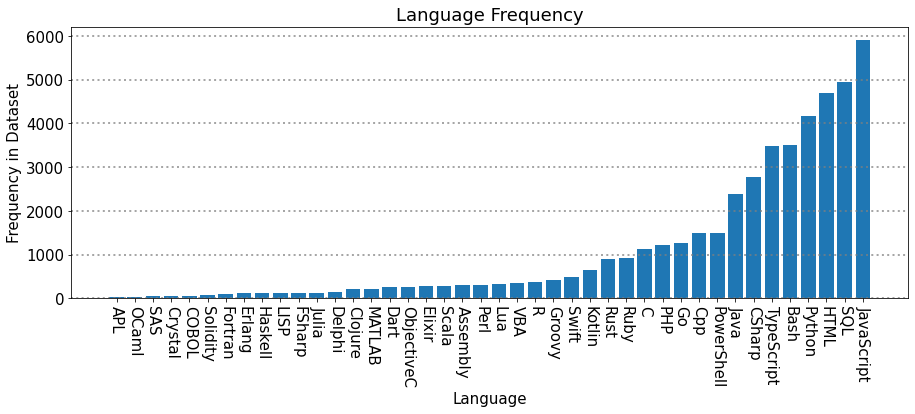
\includegraphics[width=0.9\linewidth]{frequencyLanguage.png}

\vspace{0.5in}

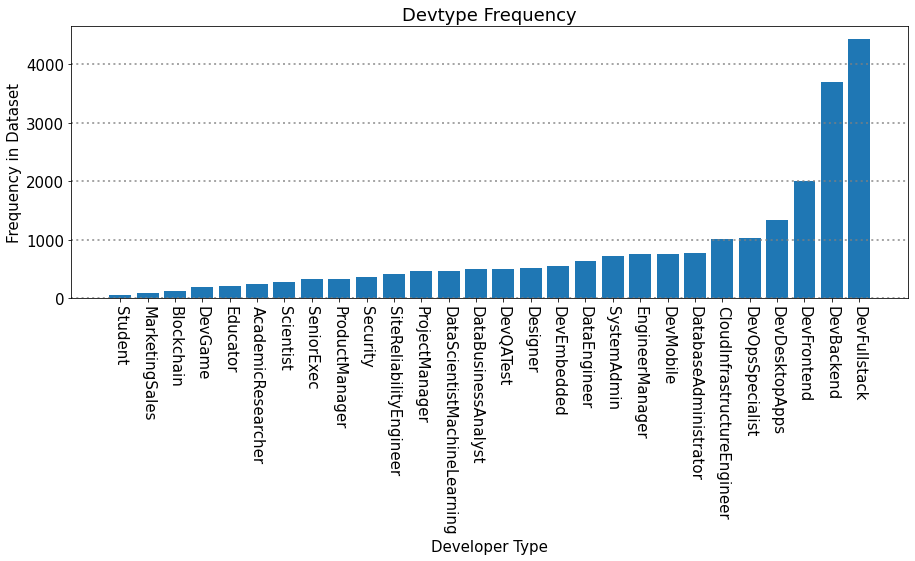
\includegraphics[width=0.9\linewidth]{frequencyDevtype.png}

\vspace{0.5in}

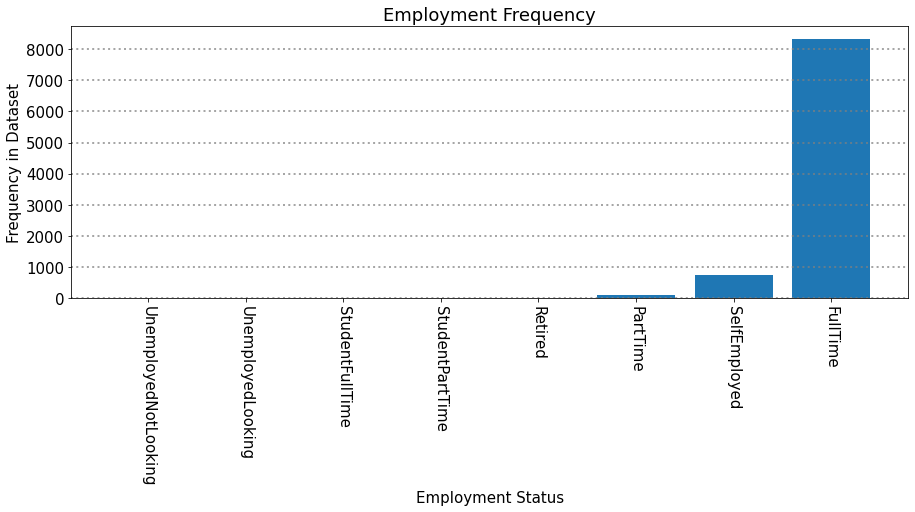
\includegraphics[width=0.9\linewidth]{frequencyEmployment.png}

\vspace{0.5in}

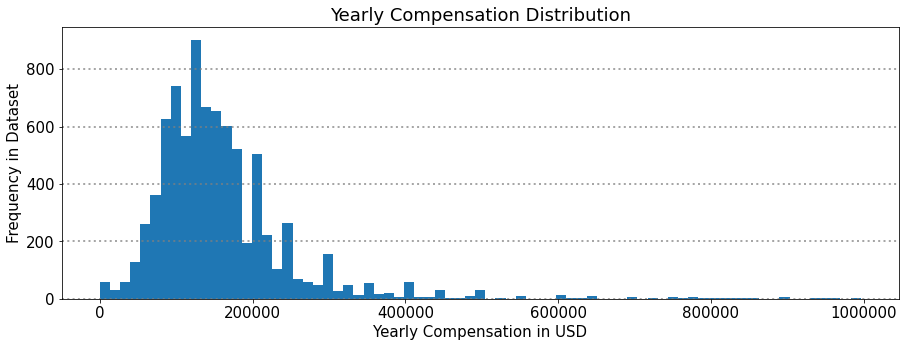
\includegraphics[width=0.9\linewidth]{frequencyConvertedCompYearly.png}

\vspace{0.5in}

These statistics will come in handy during our analysis, since it'll give us a sense of what controls may be more effective with the data.

\chapter{Analysis}

When doing analysis, I started with the basic connection, and added controls as they seemed appropriate. Each of the following sections will discuss one of those models as we approach my final conclusive model.

\section{Model Iterations}

\subsection{Model 1: The Beginning}

This is where we will start. The relationship we will look at is literally the salary when related to the coding languages used. Thus, our causal graph is very simple and basic.

\includegraphics[width=0.9\linewidth]{model1.png}

Similarly, the equation is relatively simple. Note that the summation is used to avoid needing to type out each of the language variables.

$$\log({\text{Salary}}) = \beta_0 + \sum_i{\beta_i \text{Language}_i} + \varepsilon$$

Because there is a significant number of coefficients, they have been omitted from the analysis section to prevent information being spaced out. However, you can find all of the coefficients for each model in the \hyperref[data:model1]{appendix section for Model Coefficients}.

\vspace{0.5in}

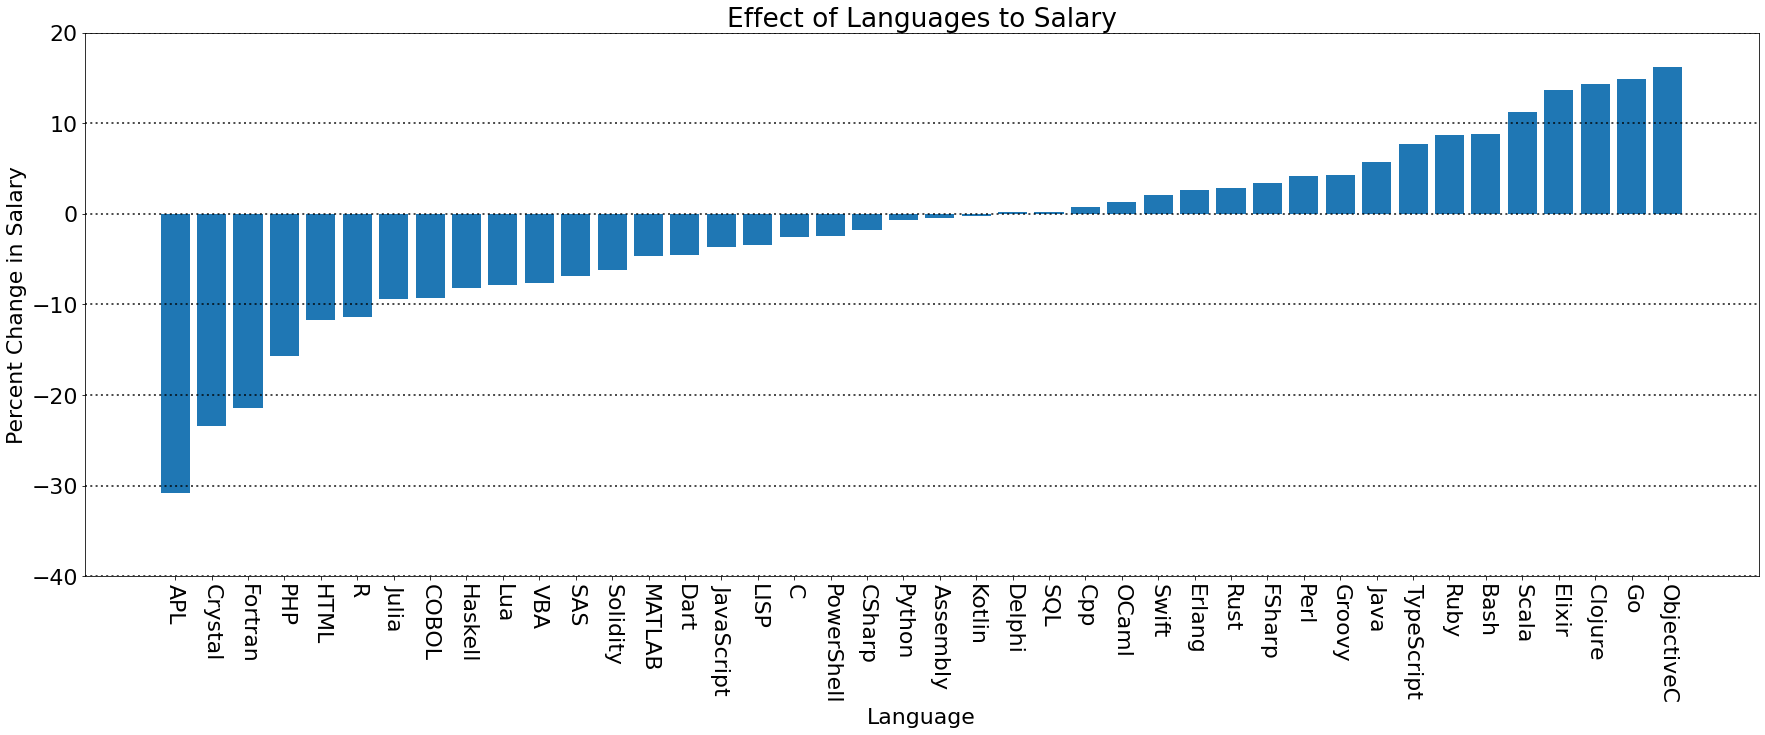
\includegraphics[width=0.9\linewidth]{model1coefficientlangauges.png}

\vspace{0.5in}

This graph shows us the relationship between working with each language and yearly salary. For example, the effect of working with HTML is $-0.1682$ or $-16.82\%$. That means that compared to the total average, if you have worked with HTML in the past year, your yearly salary would be $16.82\%$ lower. Obviously, I think there is some heteroskedasticity in this model, since we are not controlling for anything at all.

Another important measure that we should take, even if it's just to compare with future models, is the statistical significance of each coefficient. Shown below is a graph of the coefficients divided by their standard deviations. Included in the graph are lines indicating the $90\%$, $95\%$, and $99\%$ confidence interval thresholds.

\vspace{0.5in}

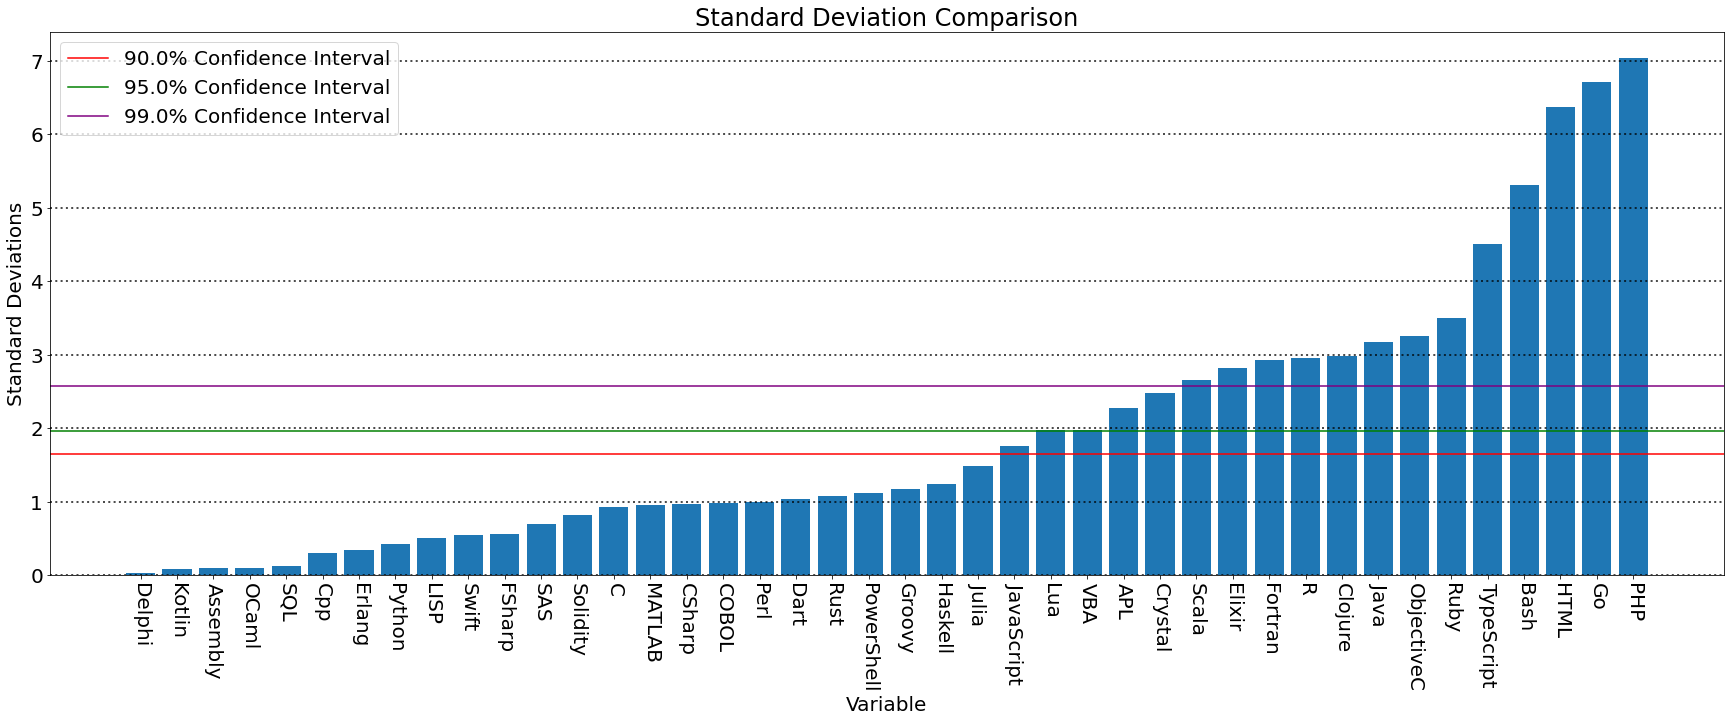
\includegraphics[width=0.9\linewidth]{model1confidencelanguages.png}

\vspace{0.5in}

As the graph indicates, very few of the coefficients are statistically significant within any of the confidence intervals. This means that only certain langauges have a significant impact on salary.

HTML is one of the most interesting ones in this model. Firstly, it is the 3rd most frequen langauge in the dataset. However, those that work in HTML have $16.82\%$ lower salaries than those who don't. And yet, HTML is one of the most statistically significant variables in this model. One potential cause could be that companies typically push tasks including HTML to interns or lower-paid employees, as it could be seen as `tedious work'.

\subsection{Model 2: Controlling for Developer Type}

Continuing with the thoughts from the previous model, I decided to control for the developer type. The developer type interacts with the system in a couple ways. First, it may indicate what languages the individual uses. For example, web developers would most likely be using HTML and Javascript. Additionally, some developer types are paid more, such as senior engineers. The implemented causal graph can be seen below:

\includegraphics[width=0.9\linewidth]{model2.png}

Similarly, our model equation will now include the Developer Types, which is once again a set of variables that will be represented in a loop

$$\log({\text{Salary}}) = \beta_0 + \sum_i{\beta_i \text{Language}_i} + \sum_j{\beta_j \text{DevType}_j} + \varepsilon$$

Once again, you can view the individual coefficients in the \hyperref[data:model2]{appendix section}. First, I looked to make sure that the deata I found for the developer types made sense.

\vspace{0.5in}

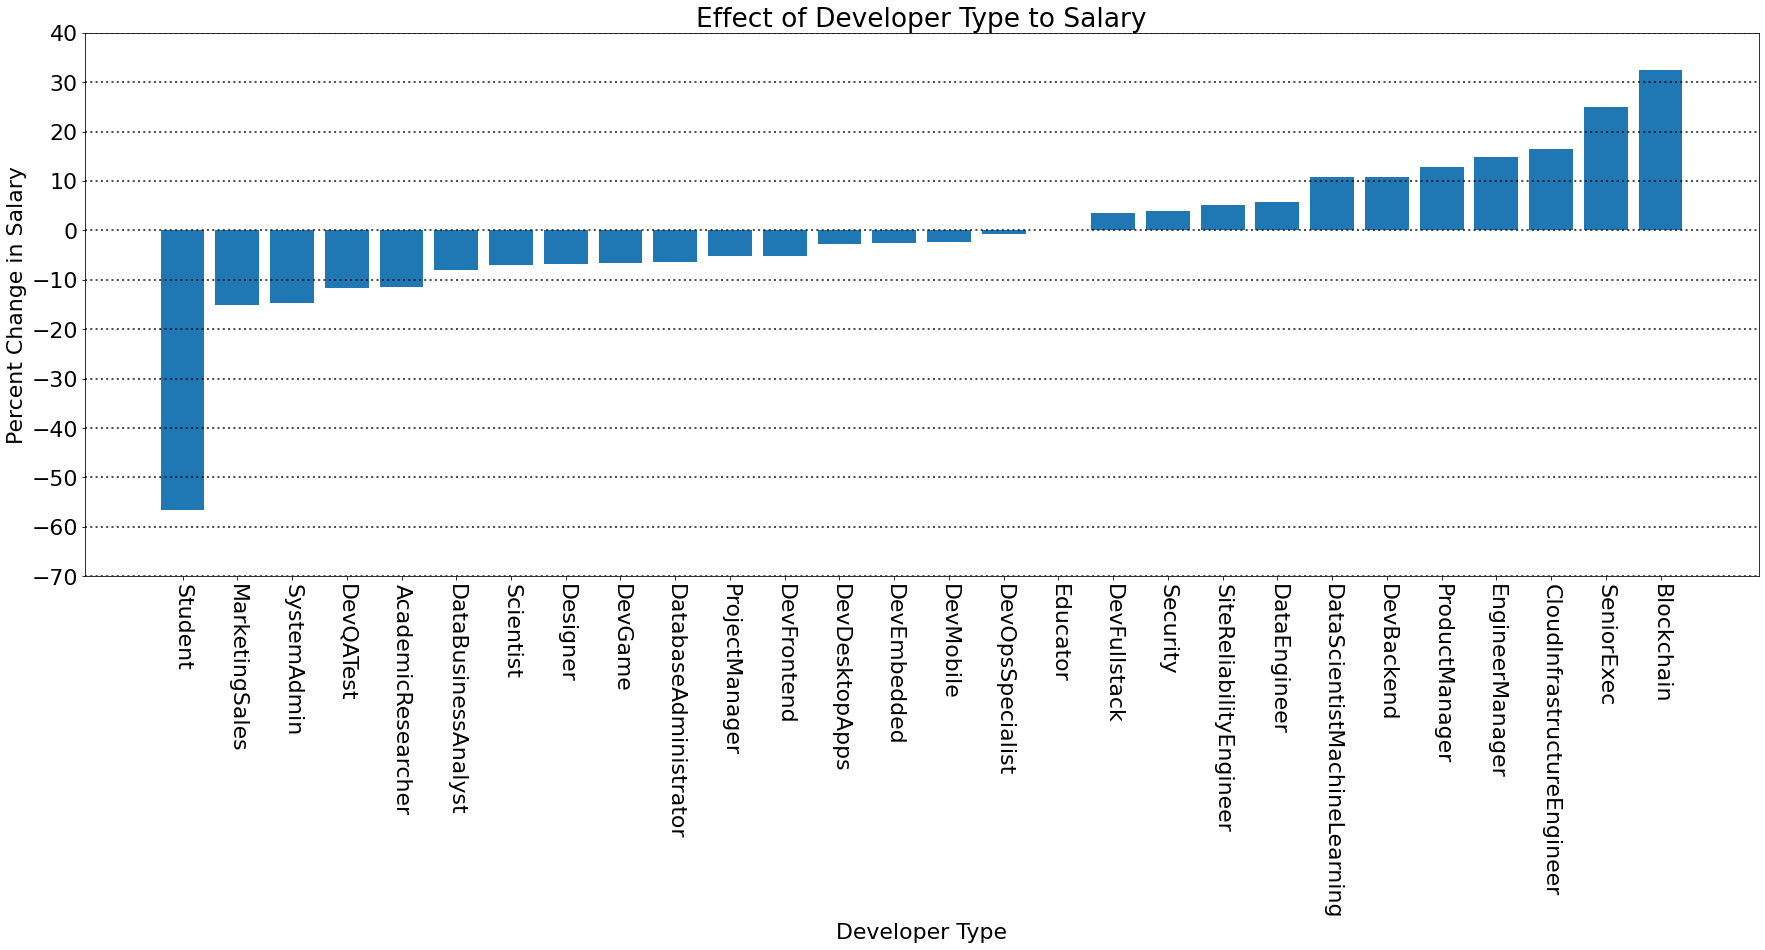
\includegraphics[width=0.9\linewidth]{model2coefficientdevtype.png}

\vspace{0.5in}

As expected, students have the largest decrease in salary. In this model, being a student means you have a $56.62\%$ lower salary than others. While in practice, I think this is much lower, it still indicates that we are going in the right direction. Additionally, Senior Executives also appear very high up. Being a Senior Executive increases your salary by $24.89\%$, according to this model.

\vspace{0.5in}

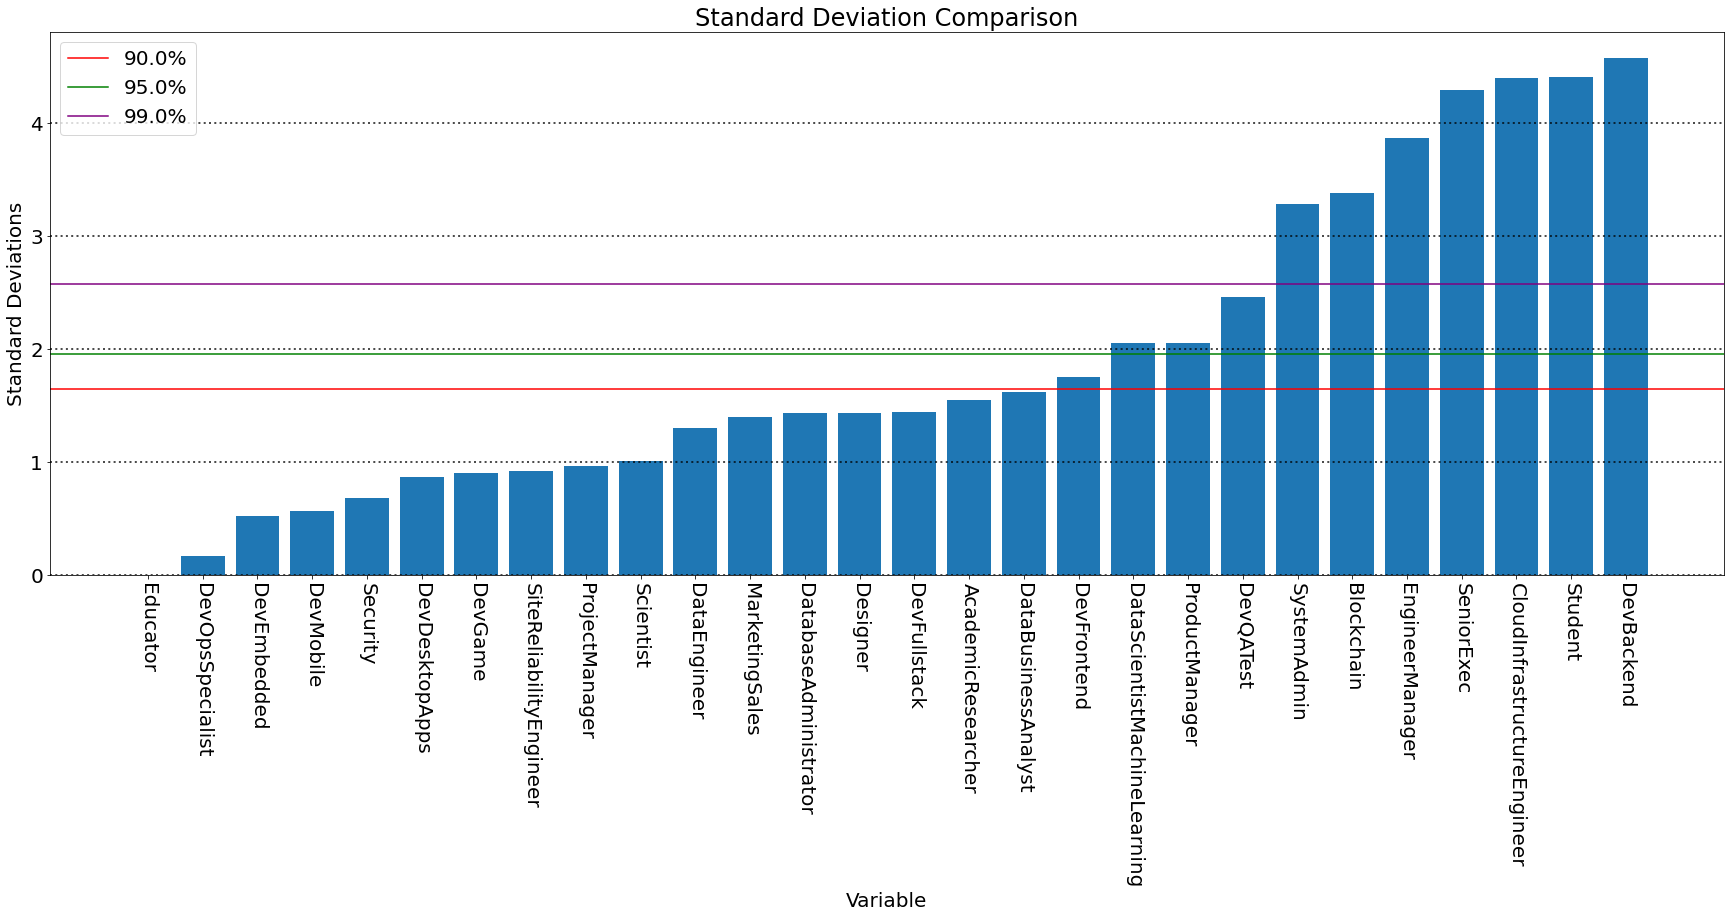
\includegraphics[width=0.9\linewidth]{model2confidencedevtype.png}

\vspace{0.5in}

If we take a look back at the dataset statistics, we see that Front End, Back End, and Full Stack take up a large majority of the dataset. However, the effect of Back End development is the only one of the three that is statistically significant under a $99\%$ confidence interval, whereas Front End is significant under a $90\%$ confidence interval.

\vspace{0.5in}

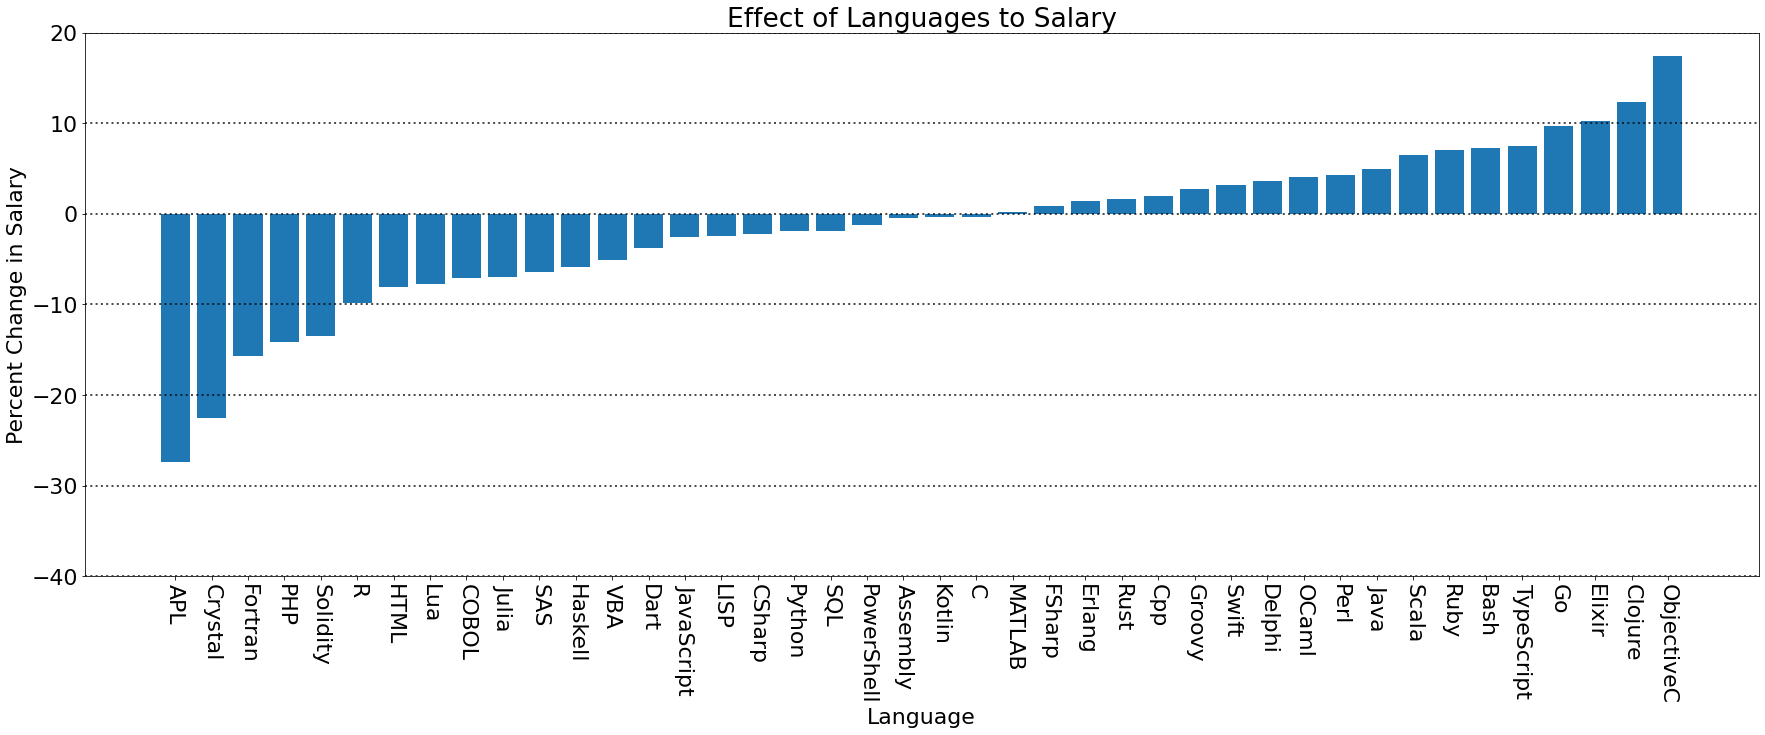
\includegraphics[width=0.9\linewidth]{model2coefficientlanguages.png}

\vspace{0.5in}

There are a few noticeable changes that happened. First, we saw Go drop from being 2nd place to 6th place, as its coefficient dropped from $13.31\%$ to $8.14\%$. The C programming language saw an increase, as it went from $-1.41\%$ to $0.92\%$. While small, that change bumped it up a good number of spots.

% The changes to the coefficients for languages hasn't changed much at all. Some have moved around, but there isn't many drastic changes. However, these minor changes seem to be going towards the right direction. For example, the coefficient on HTML increased from $-16.82\%$ to $-14.37\%$. Although it is still oddly low, it's a bit better than before.

\vspace{0.5in}

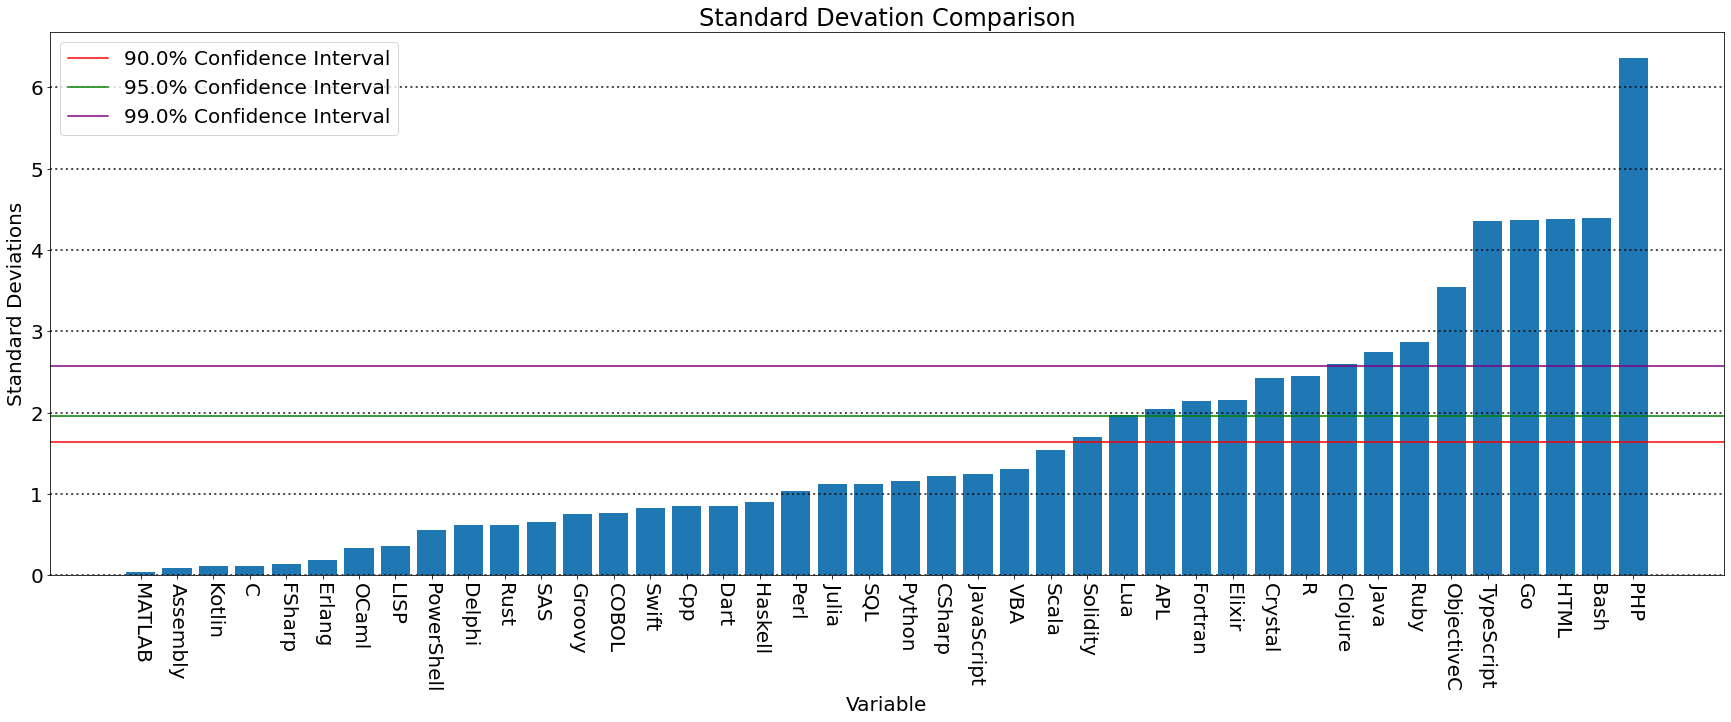
\includegraphics[width=0.9\linewidth]{model2confidencelanguages.png}

\vspace{0.5in}

The only notable change in the standard deviations is that the Go programming language, with is drastic shift in confidence interval, is no longer indicated as being significant under a $99\%$ confidence interval.

\subsection{Model 3: Controlling for Employment and Experience}

The next controls I added was for Employment Status and Work Experience. I added these together because I thought they were related enough that they would show a bit more change when together. Even though there are a lot of Employment Status variables, I decided to only include the ``FullTime'' and ``PartTime'' variables. For experience, I used the ``NumYearsCodePro'', which is the number of years that the individual has been professionally programming for. Both of these only really affect salary, so out causal graph updates accordingly.

\includegraphics[width=0.9\linewidth]{model3.png}

Similarly, our model equation now includes these constants. However, one of the important aspects to remember is that the years professionally coding is not a binary value, but a numerical value. That is, the interpretation of the number of years professionally coding is that for every additional year, the individual's salary will increase by that percent.

$$\log({\text{Salary}}) = \beta_0 + \beta_1 \text{FullTime} + \beta_2 \text{PartTime} + \beta_3 \text{YearsCodePro} + \sum_i{\beta_i \text{Language}_i} + \sum_j{\beta_j \text{DevType}_j} + \varepsilon$$

\begin{longtable}{|R{0.4\linewidth}|R{0.3\linewidth}|R{0.3\linewidth}|}
  \hline
  \textbf{Coefficient} & \textbf{Value} & \textbf{Std.Err.} \\
  \hline
  $FullTime$ & $0.24852431363579697$ & $0.05522332479437502$\\
  \hline
  $PartTime$ & $-0.38081352591020495$ & $0.11049755478678222$\\
  \hline
  $NumYearsCodePro$ & $0.012981805679194186$ & $0.0011762073012294661$ \\
  \hline
\end{longtable}

The table\footnote{I've displayed the additional constants as a table because NumYearsCodePro is not a binary value.} above shows the new variables introduced in this model\footnote{The rest of the model values can be found in its \hyperref[data:model3]{section in the appendix}}. If you divide the value by the standard error, you will find that each one is statistically signficant\footnote{Alternatively, eyeballing the values work. Notice that each value is at least triple its standard error}.

Since the NumYearsCodePro variable is not binary, its interpretation is different. This model says that for every additional year of professional coding experience you have, your salary is expected to increase by about $1.30\%$. While it may not seem much, it adds up. For example, people who have been professionally programming for about 10 years on average have around a $13\%$ higher salary.

\vspace{0.5in}

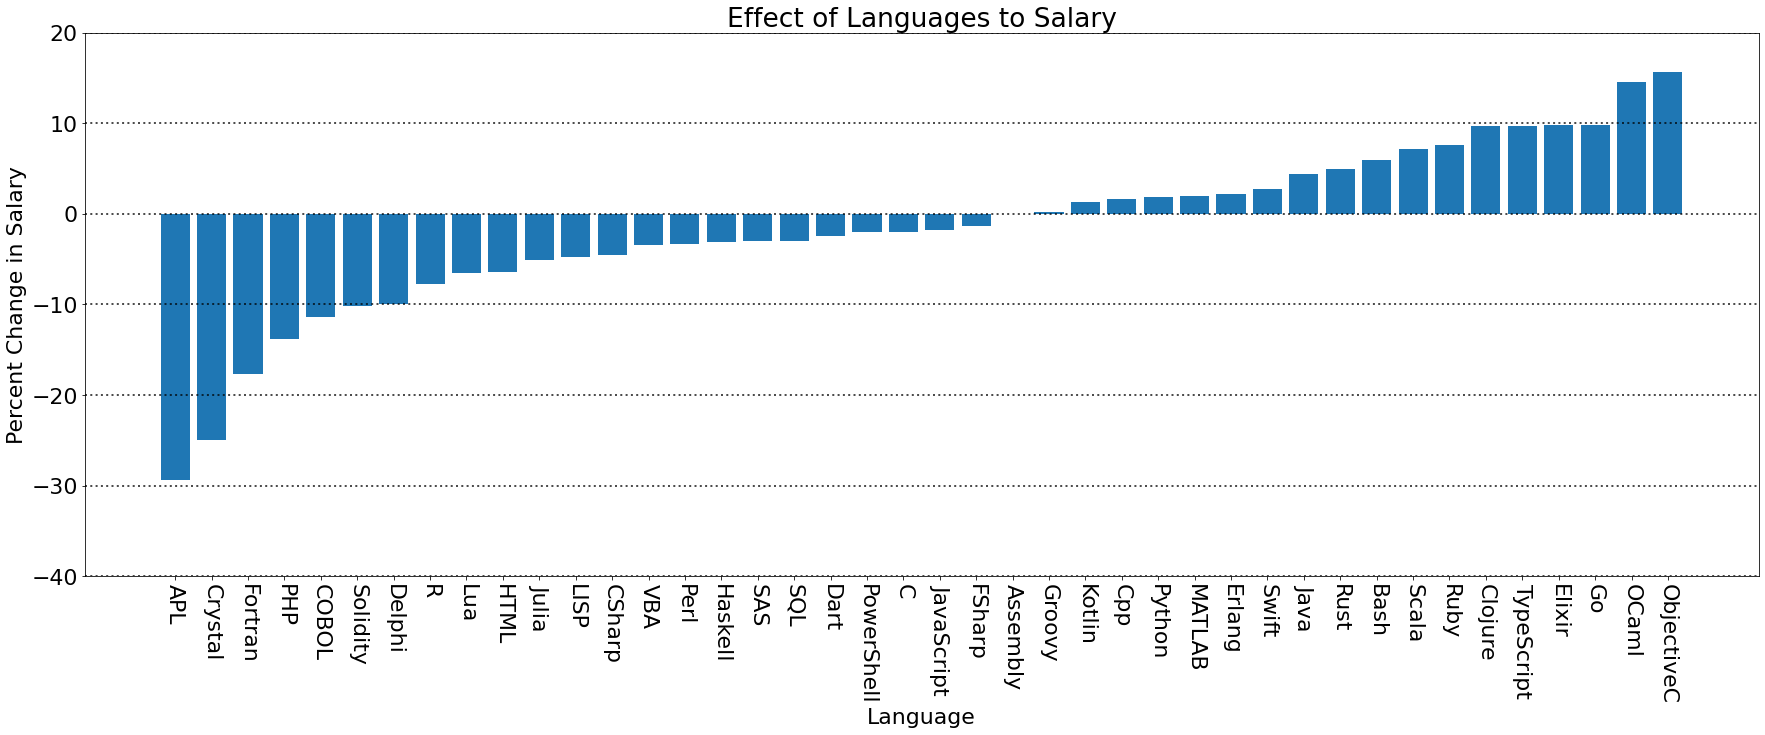
\includegraphics[width=0.9\linewidth]{model3coefficientlanguages.png}

\vspace{0.5in}

Compared to previous models, this model seems to be a lot more decisive. There are less values whose coefficients are almost zero. For example, in model 2, working with Kotlin had a measly $0.5\%$ increase in salary. However, in model 3 Kotlin increases salary by $1.79\%$, over triple the effect.

We also see some wider-recognized languages move up the list. Typescript has changed from a $9.57\%$ increase in Model 2 to a $11.35\%$ increase. Rust also jumped from close to the middle with a $4.02\%$ up to the top 5 with $6.8\%$.

\vspace{0.5in}

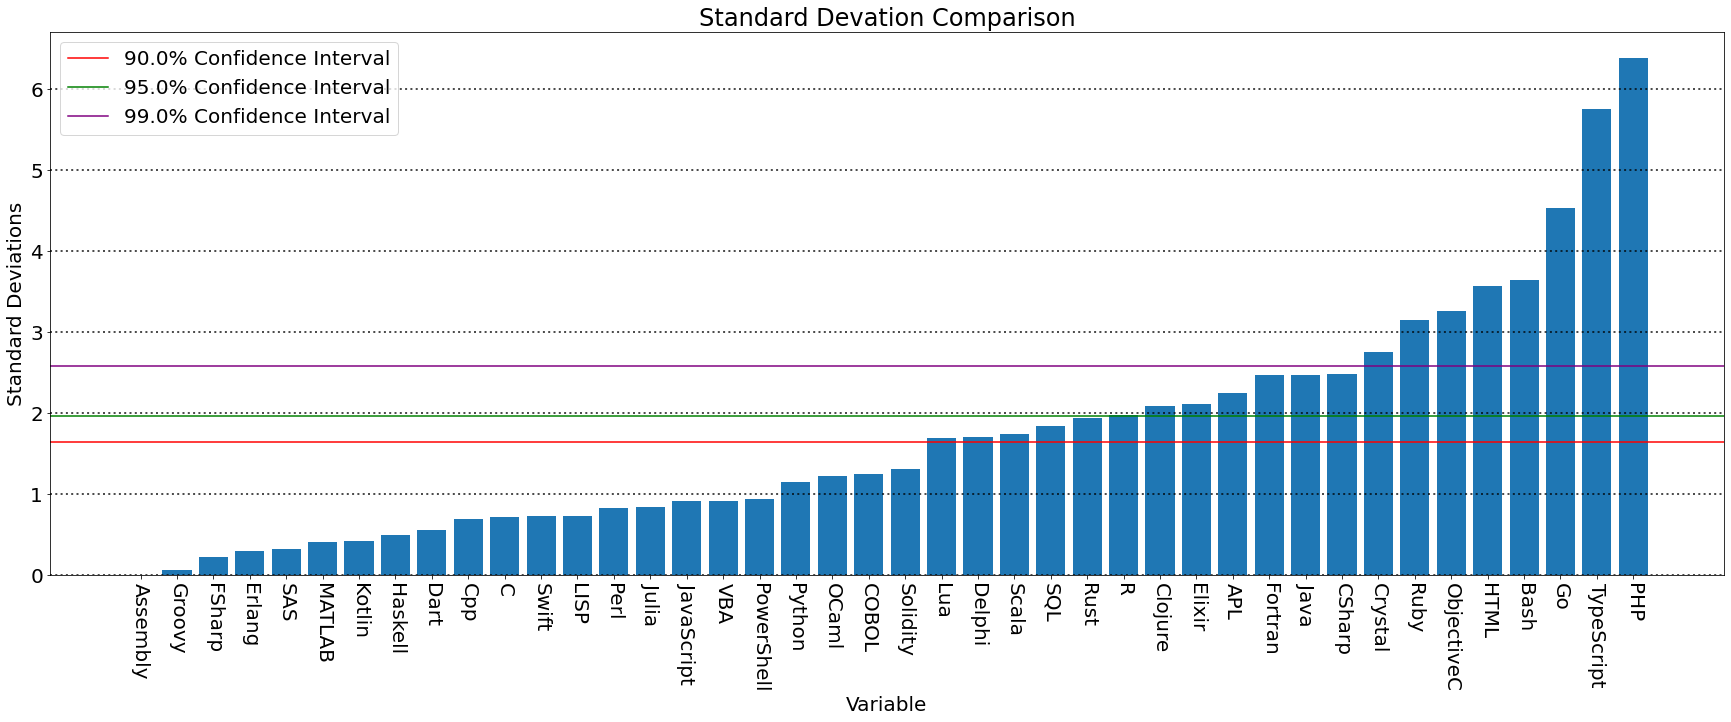
\includegraphics[width=0.9\linewidth]{model3confidencelanguages.png}

\vspace{0.5in}

The changes in the coefficients also reflect in the changes in standard deviation. Our examples of Typescript and Rust both reflect in confidence intervals. In fact, Rust is now indicated to be statistically significant under a $90\%$ confidence interval.


\newpage
\section{The Finalized Model}

The final model that we'll use to analyze is Model 3. As a refresher, this model is controlling for deeveloper type, employment status, and years of professional coding experience. The results from this model are pretty surprising, and not at all what I expected to get.

$$\log({\text{Salary}}) = \beta_0 + \beta_1 \text{FullTime} + \beta_2 \text{PartTime} + \beta_3 \text{YearsCodePro} + \sum_i{\beta_i \text{Language}_i} + \sum_j{\beta_j \text{DevType}_j} + \varepsilon$$

The final variables for this model can be found in \hyperref[data:model3]{the appendix for model 3's coefficients}.

\vspace{0.5in}

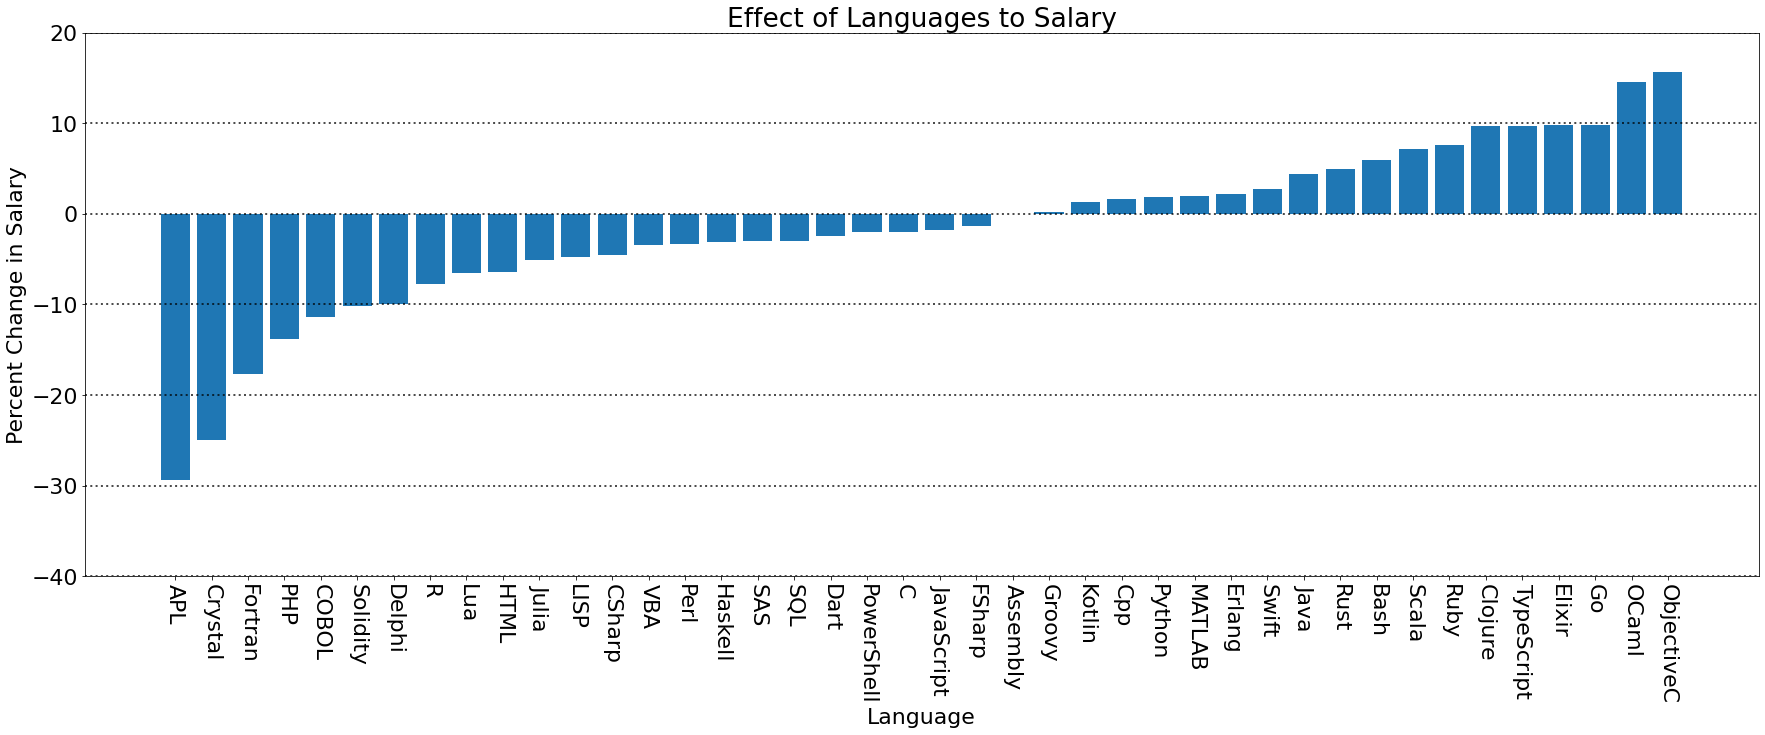
\includegraphics[width=0.9\linewidth]{model3coefficientlanguages.png}

\vspace{0.5in}

For each language listed on the graph, the value indicates the relative to the salary. For example, the coefficient on R is $-0.0419$. This means that someone who uses R has an average salary $4.19\%$ lower than someone who does not use R. This seems counterintuitive, but it makes sense in application.

\vspace{0.5in}

\includegraphics[width=0.9\linewidth]{model3coefficientdevtypes.png}

\vspace{0.5in}





\end{document}
